% Options for packages loaded elsewhere
\PassOptionsToPackage{unicode}{hyperref}
\PassOptionsToPackage{hyphens}{url}
%
\documentclass[
  12pt,
]{article}
\title{Temporal and Spatial Trends in Adaptation to Flooding in the
United States}
\usepackage{etoolbox}
\makeatletter
\providecommand{\subtitle}[1]{% add subtitle to \maketitle
  \apptocmd{\@title}{\par {\large #1 \par}}{}{}
}
\makeatother
\subtitle{\url{https://github.com/maggieoshea/OSheaPearceSanchez_ENV872_EDA_FinalProject.git}}
\author{Maggie O'Shea, Garrett Pearce, and Diane Sanchez}
\date{}

\usepackage{amsmath,amssymb}
\usepackage{lmodern}
\usepackage{iftex}
\ifPDFTeX
  \usepackage[T1]{fontenc}
  \usepackage[utf8]{inputenc}
  \usepackage{textcomp} % provide euro and other symbols
\else % if luatex or xetex
  \usepackage{unicode-math}
  \defaultfontfeatures{Scale=MatchLowercase}
  \defaultfontfeatures[\rmfamily]{Ligatures=TeX,Scale=1}
  \setmainfont[]{Times New Roman}
\fi
% Use upquote if available, for straight quotes in verbatim environments
\IfFileExists{upquote.sty}{\usepackage{upquote}}{}
\IfFileExists{microtype.sty}{% use microtype if available
  \usepackage[]{microtype}
  \UseMicrotypeSet[protrusion]{basicmath} % disable protrusion for tt fonts
}{}
\makeatletter
\@ifundefined{KOMAClassName}{% if non-KOMA class
  \IfFileExists{parskip.sty}{%
    \usepackage{parskip}
  }{% else
    \setlength{\parindent}{0pt}
    \setlength{\parskip}{6pt plus 2pt minus 1pt}}
}{% if KOMA class
  \KOMAoptions{parskip=half}}
\makeatother
\usepackage{xcolor}
\IfFileExists{xurl.sty}{\usepackage{xurl}}{} % add URL line breaks if available
\IfFileExists{bookmark.sty}{\usepackage{bookmark}}{\usepackage{hyperref}}
\hypersetup{
  pdftitle={Temporal and Spatial Trends in Adaptation to Flooding in the United States},
  pdfauthor={Maggie O'Shea, Garrett Pearce, and Diane Sanchez},
  hidelinks,
  pdfcreator={LaTeX via pandoc}}
\urlstyle{same} % disable monospaced font for URLs
\usepackage[margin=2.54cm]{geometry}
\usepackage{graphicx}
\makeatletter
\def\maxwidth{\ifdim\Gin@nat@width>\linewidth\linewidth\else\Gin@nat@width\fi}
\def\maxheight{\ifdim\Gin@nat@height>\textheight\textheight\else\Gin@nat@height\fi}
\makeatother
% Scale images if necessary, so that they will not overflow the page
% margins by default, and it is still possible to overwrite the defaults
% using explicit options in \includegraphics[width, height, ...]{}
\setkeys{Gin}{width=\maxwidth,height=\maxheight,keepaspectratio}
% Set default figure placement to htbp
\makeatletter
\def\fps@figure{htbp}
\makeatother
\setlength{\emergencystretch}{3em} % prevent overfull lines
\providecommand{\tightlist}{%
  \setlength{\itemsep}{0pt}\setlength{\parskip}{0pt}}
\setcounter{secnumdepth}{5}
\usepackage{booktabs}
\usepackage{longtable}
\usepackage{array}
\usepackage{multirow}
\usepackage{wrapfig}
\usepackage{float}
\usepackage{colortbl}
\usepackage{pdflscape}
\usepackage{tabu}
\usepackage{threeparttable}
\usepackage{threeparttablex}
\usepackage[normalem]{ulem}
\usepackage{makecell}
\usepackage{xcolor}
\usepackage{amsmath}
\usepackage{caption}
\ifLuaTeX
  \usepackage{selnolig}  % disable illegal ligatures
\fi

\begin{document}
\maketitle

\hypertarget{left-to-do}{%
\section{Left to do:}\label{left-to-do}}

\begin{itemize}
\tightlist
\item
  Figure out a way to get the table names into the table of contents
\item
  Figure out why the figures are knitting in the wrong place
\end{itemize}

\newpage
\tableofcontents 
\newpage
\listoftables

1Selected Flooding Adaptation Type Codes\\
\newline
2 FEMA Hazard Mitigated Properties Dataset: Summary Statistics\\
\newline
3 Results from Time Series Analysis of All Adaptation Types\\
\newline
4 Results from Time Series Analysis of Ex-Situ Adaptation\\
\newline
5 Results from Time Series Analysis of In-Situ Adaptation\\
\newpage

\listoffigures 
\newpage

\newpage

\hypertarget{rationale-and-research-questions}{%
\section{Rationale and Research
Questions}\label{rationale-and-research-questions}}

Extreme weather events and natural disasters seem to be on the rise
worldwide, and climate adaptation is vital to communities at risk. In
the U.S., flooding is the most common natural disaster with the cost of
flooding in the United States in 2020 estimated at \$32.1 billion (IDMC
2019, Lindsey 2022, Wing et al.~2022). These costs, both financial as
well as social, are expected to only rise as there is a predicted 24\%
increase in flooding by 2050 (Wing et al.~2022). Already, regions in the
United States are seeing drastic increases in flooding since the 1950s -
a study by the United States Environmental Protection Agency on 33 sites
around the United States found flooding to be at least five times more
common in over half the areas studies, with a strong concentration in
sites along the eastern seaboard (EPA 2022). Given the rapid increase in
flooding around the United States as well as the severe impacts this
hazard can have, adaptation is becoming increasingly important and
resources that already exist for these efforts are likely to become more
strained.

It will be increasingly important to understand the resources that are
already available to communities, the accessibility of these resources,
as well as how they are being used. This analysis seeks to uncover some
of this through examining the trends in flood mitigation assistance
provided by the Federal Emergency Management Agency. A time series
analysis helped to identify possible trends in the number of grants
received for flooding over time as well as the amount paid by FEMA to
understand if trends in the use of these resources are similarly
increasing as flooding has been. Furthermore, due to the drastic impacts
of flooding that are only increasing, we were interested to examine if
individuals are relying more heavily on ex-situ adaptation measures to
move away from these hazards, or if communities are attempting to stay
where they are despite the flooding and thus relying on in-situ
adaptation measures. The research questions that guided this work were:

\begin{enumerate}
\def\labelenumi{\arabic{enumi}.}
\tightlist
\item
  Are there trends in the number of properties that received grants to
  adapt to flooding in the United States over time?
\item
  Are there trends in the amount FEMA paid for hazard mitigation for
  flooding over time?
\item
  How do these trends differ for in-situ vs ex-situ adaptation?
\end{enumerate}

The temporal scale of the research was defined by the FEMA Mitigated
Properties dataset which included information on grants from 1985 until
2020 allowing the time series analysis to cover a 35 year time-frame.
The grants included those received in all states in the United States.
This analysis also included a brief spatial analysis focusing on one
state in particular to spatially visualize the data as well as examine
potential spatial trends in ex-situ vs.~in-situ adaptation funding.

\newpage

\hypertarget{dataset-information}{%
\section{Dataset Information}\label{dataset-information}}

\hypertarget{dataset-background-and-retrieval}{%
\subsection{2.1 Dataset Background and
Retrieval:}\label{dataset-background-and-retrieval}}

We used data managed by the Federal Emergency Management Agency's
National Emergency Management Information Systems, downloaded directly
in a CSV format through FEMA's OpenFEMA resource. The dataset includes
the record of properties that received grant assistance for hazard
mitigation through any of the Hazard Mitigation Assistance grant
programs, programs administered by FEMA that seek to reduce losses from
disasters as well as protect life and property in the face of hazards
(FEMA 2022). This includes: the Hazard Mitigation Grant Program, the
Flood Mitigation Assistance Grant Program, and the Pre-Disaster
Mitigation Grant Program (ibid.). Entries prior to 2012 also include
grants received through the Repetitive Flood Claims Grant program and
Severe Repetitive Loss Grant Program which both were eliminated through
the Biggert Water Flood Insurance Reform Act of 2012 (ibid.). Each entry
includes data such as the total amount paid, the number of properties
receiving support, the hazard that the grant is adapting against, the
program year, and others. The variables we used in particular were:
Total Amount Paid per grant, Number of Properties per grant, Program
Year, and the county where the grant was funded. These were wrangled and
summed for our analysis.

For the spatial analysis, the county boundaries for North Carolina were
downloaded from the OpenESRI platform which had the State of North
Carolina's Emergency Management Agency's best current available data as
of 2020. These boundaries were identified through sources including the
North Carolina Geodetic Survey, the North Carolina Department of
Transportation, the United States Geological Survey, as well as field
surveys that have been recorded by the respective county (State of North
Carolina 2020).

\hypertarget{data-wrangling}{%
\subsection{2.2 Data Wrangling}\label{data-wrangling}}

The mitigated properties dataset required three different types of
wrangling for the analysis. First, we wrangled the data to result in a
dataset with the total number of properties that received a grant for
any type of flooding adaptation and the total amount paid for these per
year. Second, we wrangled the data to have this same information, number
of properties and total amount paid, for ex-situ adaptation, or buyouts,
per year and did the same for in-situ adaptation. Finally, we wrangled
the mitigated properties dataset in the same ways - finding number of
properties and total amount paid for all flooding grants, ex-situ
grants, and in-situ grants but instead of summarizing per year, we
selected for only North Carolina grants and grouped the data by county
for our spatial analysis.

\newpage

\emph{Table 1: Selected Flooding Adaptation Type Codes}

\captionsetup[table]{labelformat=empty,skip=1pt}
\setlength{\LTpost}{0mm}
\begin{longtable}{ll}
\caption*{
{\large Mitigated Properties Flooding Type Codes}
} \\ 
\toprule
Code & Activity \\ 
\midrule
\multicolumn{1}{l}{In-Situ Adaptation} \\ 
\midrule
202.1 & Elevation of Private Structures—Riverine \\ 
202.2 & Elevation of Private Structures—Coastal \\ 
202.3 & Elevation of Public Structures—Riverine \\ 
202.4 & Elevation of Public Structures—Coastal \\ 
203.1 & Wet Floodproofing Private Structures—Riverine \\ 
203.2 & Wet Floodproofing Private Structures—Coastal \\ 
203.3 & Wet Floodproofing Public Structures—Riverine \\ 
203.4 & Wet Floodproofing Public Structures—Coastal \\ 
204.1 & Dry Floodproofing Private Structures—Riverine (Commercial) \\ 
204.2 & Dry Floodproofing Private Structures—Coastal (Commercial) \\ 
204.3 & Dry Floodproofing Public Structures—Riverine \\ 
204.4 & Dry Floodproofing Public Structures—Coastal \\ 
204.5 & Dry Floodproofing Private Structures—Riverine (Residential-Historic) \\ 
204.6 & Dry Floodproofing Private Structures—Coastal (Residential-Historic) \\ 
207.2 & Mitigation Reconstruction \\ 
\midrule
\multicolumn{1}{l}{Ex-Situ Adaptation} \\ 
\midrule
200.1 & Acquisition of Private Real Property (Structures and Land)—Riverine \\ 
200.2 & Acquisition of Private Real Property (Structures and Land)—Coastal \\ 
200.3 & Acquisition of Public Real Property (Structures and Land)—Riverine \\ 
200.4 & Acquisition of Public Real Property (Structures and Land)—Coastal \\ 
200.5 & Acquisition of Vacant Land \\ 
201.1 & Relocation of Private Structures—Riverine \\ 
201.2 & Relocation of Private Structures—Coastal \\ 
201.3 & Relocation of Public Structures—Riverine \\ 
201.4 & Relocation of Public Structures—Coastal \\ 
\bottomrule
\end{longtable}
\begin{minipage}{\linewidth}
Source: Open FEMA Dataset\\
\end{minipage}

In order to do so, we first examined and explored the dataset and found
that some entries had a total amount paid that was negative. Because the
OpenFEMA information page included a note that these were manually
entered data and subject to human error, we made the assumption that
this was due to human error and removed these negative values from our
analysis. After doing so, we used this cleaned mitigated properties
dataset to create our three different types of wrangled datasets. This
involved, first, examining the ``type'' codes to identify which type
codes indicate that the grants were used for flooding. Table 1 shows the
type codes that were used, grouped by ex-situ and in-situ codes. These
type codes together were used to find all flooding grants regardless of
adaptation type.

After selecting out the relevant flooding type codes, we grouped by year
or county and summarized the datasets to find the sum of the number of
properties and the total amount paid for each category we were examining
in this analysis (amount paid for all flooding grants per year, amount
paid for ex-situ grants per year, etc.).For the total amount paid
categories specifically, using the ``priceR'' package, we adjusted each
of the total amount paid values per year for all adaptation, ex-situ,
and in-situ for inflation. Summary statistics for the respective
wrangled datasets can be found in table 2.

\emph{Table 2: FEMA Hazard Mitigated Properties Dataset: Summary
Statistics}\\
\captionsetup[table]{labelformat=empty,skip=1pt}
\setlength{\LTpost}{0mm}

\begin{longtable}{lcrrr}
\caption*{
{\large \textbf{Administration of Hazard Mitigation Grants}}
} \\ 
\toprule
Category & Observations & Mean & Median & SD \\ 
\midrule
\multicolumn{1}{l}{\emph{\textbf{All Adaptation}}} \\ 
\midrule
Total Number of Properties & $32$ & $2,045.84$ & $1,733.00$ & $1,842$ \\ 
Total Amount Paid (\$) & $32$ & $219,422,363.28$ & $41,158,369.00$ & $416,423,807$ \\ 
\midrule
\multicolumn{1}{l}{\emph{\textbf{In-Situ Adaptation}}} \\ 
\midrule
In-Situ Number of Properties & $32$ & $500.41$ & $310.00$ & $732$ \\ 
In-Situ Amount Paid (\$) & $32$ & $31,647,790.59$ & $348,242.00$ & $145,080,428$ \\ 
\midrule
\multicolumn{1}{l}{\emph{\textbf{Ex-Situ Adaptation}}} \\ 
\midrule
Ex-Situ Number of Properties & $32$ & $1,599.12$ & $1,227.00$ & $1,643$ \\ 
Ex-Situ Amount Paid (\$) & $32$ & $214,819,450.59$ & $39,533,213.00$ & $415,722,662$ \\ 
\bottomrule
\end{longtable}
\begin{minipage}{\linewidth}
Source: Open FEMA Dataset\\
\end{minipage}

\newpage

\hypertarget{exploratory-analysis}{%
\section{Exploratory Analysis}\label{exploratory-analysis}}

After wrangling the data, we explored the data both over time as well as
totals for the number of properties and amount paid in our dataset,
compared between all flooding and ex-situ vs.~in-situ. Figure 1 shows
the differences in the total number of properties between 1985 and 2020
that received adaptation flooding, comparing all of the properties with
ex-situ and in-situ. The graph shows that more properties received
ex-situ than in-situ grants by a considerable amount.

\begin{figure}
\centering
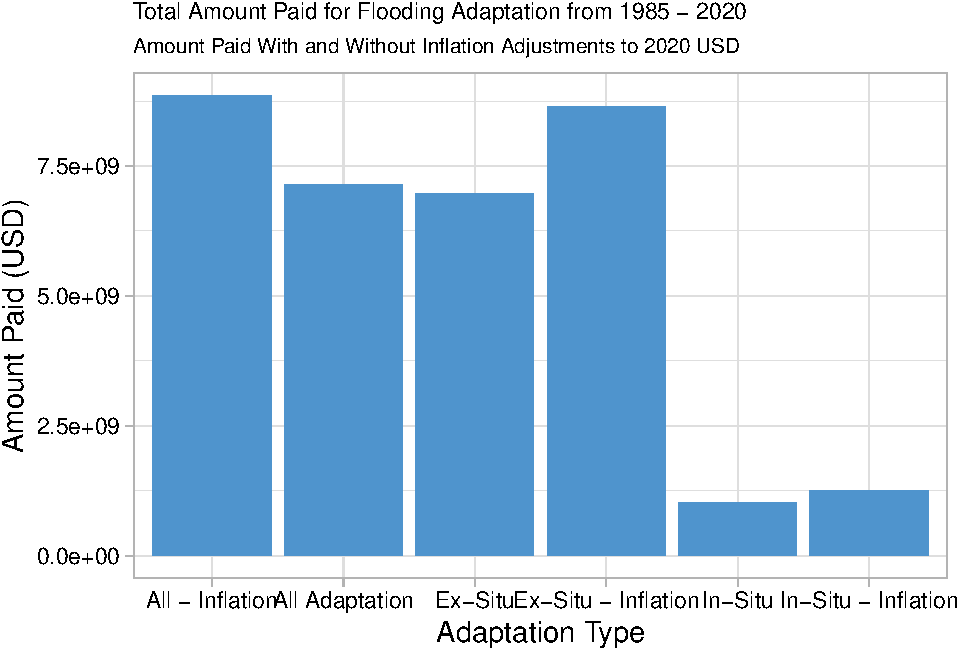
\includegraphics{finalreport_files/figure-latex/unnamed-chunk-6-1.pdf}
\caption{Total Properties that Received Flood Adaptation Funding from
1985 to 2020}
\end{figure}

\newpage

To examine this relationship further, we compared the total amount paid
for all adaptation types and in-situ vs.~ex-situ in Figure 2. In
including both the total amount paid as reported by FEMA as well as
these values adjusted to 2020 dollars, this figure helps to also show
the difference that inflation makes in the resulting total amount paid.
\newline

\begin{figure}
\centering
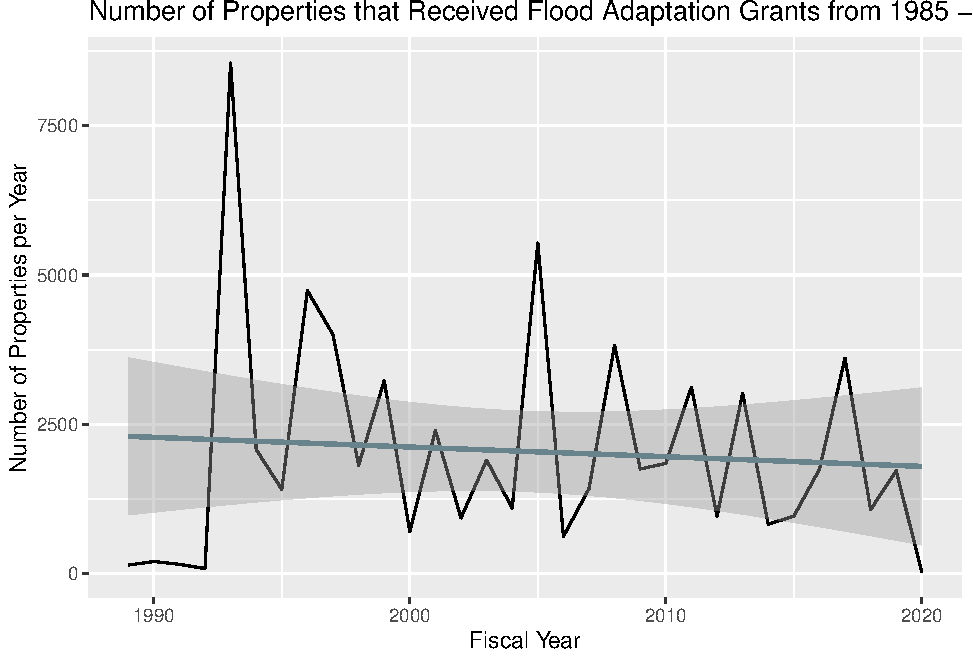
\includegraphics{finalreport_files/figure-latex/unnamed-chunk-7-1.pdf}
\caption{Total Amount Paid for Flooding Adaptation from 1985 - 2020}
\end{figure}

Finally, figures 3 and 4 show this same data over time. Figure 3 shows
the number of properties that received flood adaptation grants per year
between 1985 and 2020. \newline

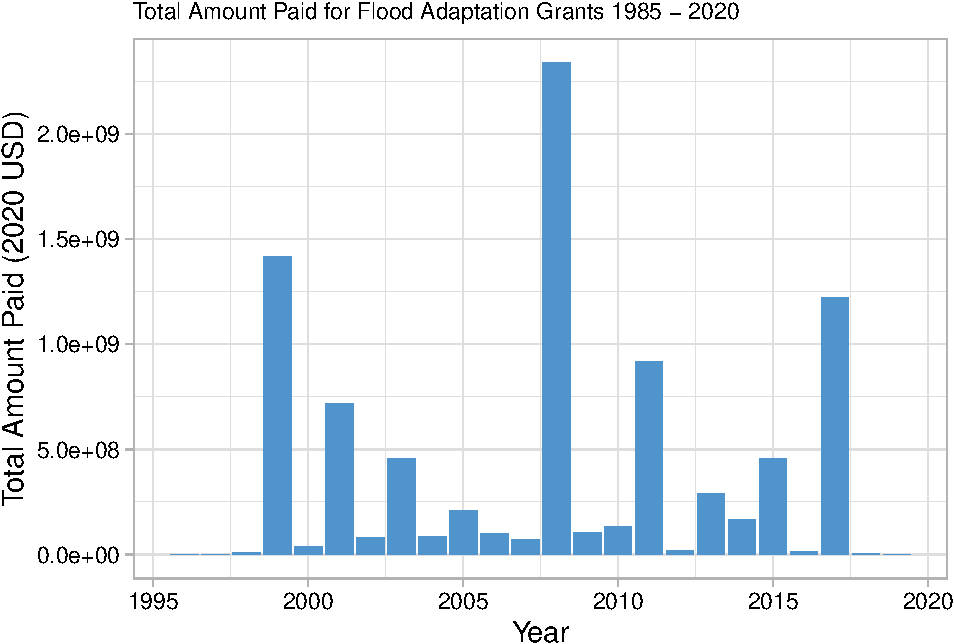
\includegraphics{finalreport_files/figure-latex/unnamed-chunk-8-1.pdf}
\newpage

Figure 4 shows the total amount paid by FEMA through flood adaptation
grants per year between 1985 and 2020. \newline

\begin{figure}
\centering
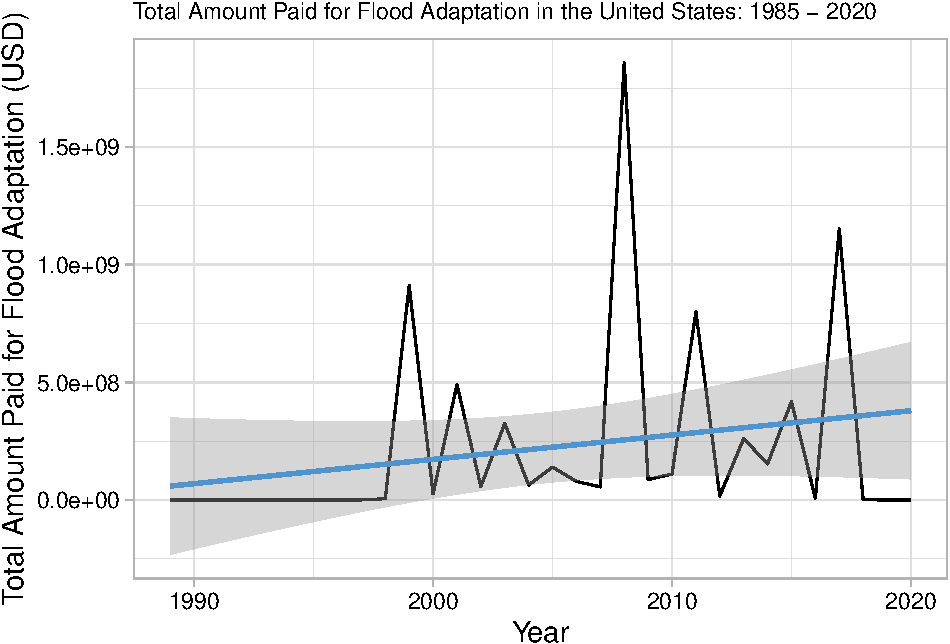
\includegraphics{finalreport_files/figure-latex/unnamed-chunk-9-1.pdf}
\caption{Total Amount Paid for Flood Adaptation Grants from 1985 to 2020
in 2020 inflation adjusted U.S. dollars}
\end{figure}

These graphs, as well as the graphs of ex-situ and in-situ data over
time, are further examined in the analysis section including trend-lines
to complement the time series analysis.

\newpage

\hypertarget{analysis}{%
\section{Analysis}\label{analysis}}

This analysis involved nine time series analysis which all sought to
examine monotonic trends over time in the number of properties receiving
grant funding for flooding adaptation and the total amount paid for
flooding adaptation from these grants. These nine analysis can be
understood based on the questions that each time series helps to answer:

\textbf{\emph{All Adaptation}}

\begin{itemize}
\item
  Total Number of Properties: Is there a monotonic trend in the total
  number of properties that receive grant funding over time?
\item
  Total Amount Paid for All Adaptation: Is there a monotonic trend in
  the total amount paid for flooding adaptation grants over time?
\item
  Total Amount Paid - Inflation Adjusted: Is there (still) a monotonic
  trend in the total amount paid for flooding adaptation grants over
  time when adjusting for inflation to 2020 dollars?
\end{itemize}

\textbf{\emph{Ex-Situ Adaptation}}

\begin{itemize}
\item
  Number of Buyouts: Is there a monotonic trend in the total number of
  properties that received ex-situ grant funding, or funding to buyout
  the property, over time?
\item
  Amount Paid for Buyouts: Is there a monotonic trend in the amount paid
  for buyouts over time?
\item
  Amount Paid for Buyouts - Inflation Adjusted: Is there (still) a
  monotonic trend in the amount paid for buyouts after adjusting for
  inflation to 2020 dollars?
\end{itemize}

\textbf{\emph{In-Situ Adaptation}}

\begin{itemize}
\item
  Number of In-Situ Properties: Is there a monotonic trend in the total
  number of properties that received in-situ grant funding to adapt in
  place over time?
\item
  Amount Paid for In-Situ Adaptation: Is there a monotonic trend in the
  amount paid for in-situ adaptation over time?
\item
  Amount Paid for In-Situ Adaptation - Inflation Adjusted: Is there
  (still) a monotonic trend in the amount paid for in-situ adaptation
  after adjusting for inflation to 2020 dollars?
\end{itemize}

These data were also visualized through a spatial analysis of the number
of properties and total amount paid for flood adaptation grants in North
Carolina including for all grants, ex-situ grants, and in-situ grants.

\hypertarget{all-adaptation-types}{%
\subsection{4.1 All Adaptation Types}\label{all-adaptation-types}}

Beginning with the analysis of all adaptation types, overall the only
statistically significant monotonic trend found was the trend in the
total amount paid for flood adaptation in the United States, before
adjusting for inflation. The total number of properties that received
adaptation funding from 1985 to 2020 did not have a statistically
significant monotonic trend (p \textgreater{} 0.9) which is evident in
figure 5 which shows the number of properties over time as well as the
associated trend line.

\begin{figure}
\centering
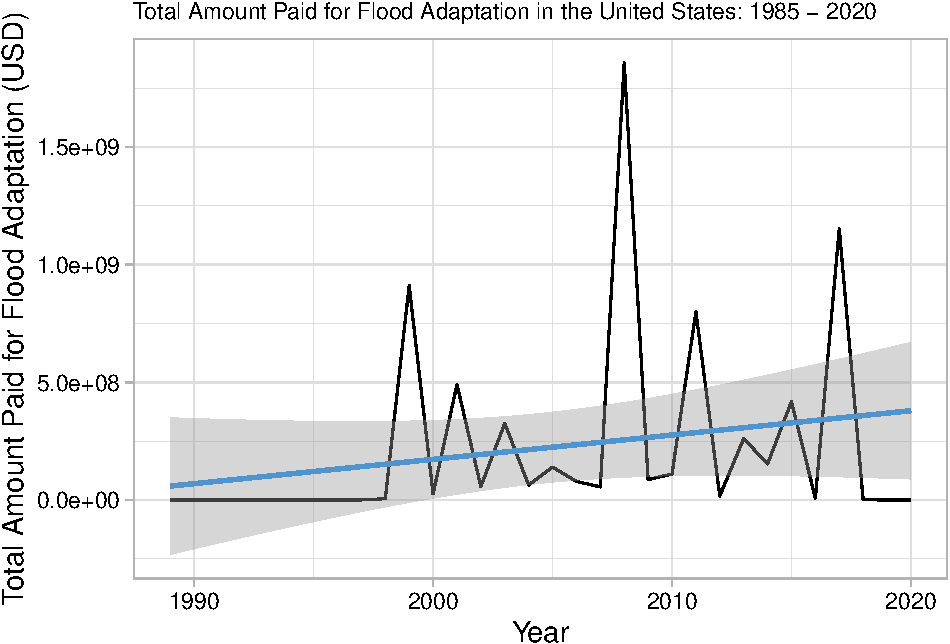
\includegraphics{finalreport_files/figure-latex/unnamed-chunk-10-1.pdf}
\caption{Number of Properties that Received Flood Adaptation Grants
between 1985 and 2020}
\end{figure}

The second time series analysis which was statistically significant (p =
0.004), showed an increasing trend (tau = 0.361) in the total amount
paid over time for flood adaptation through FEMA. Figure 6 shows this
data over time with the associated trend line. \newpage

\begin{figure}
\centering
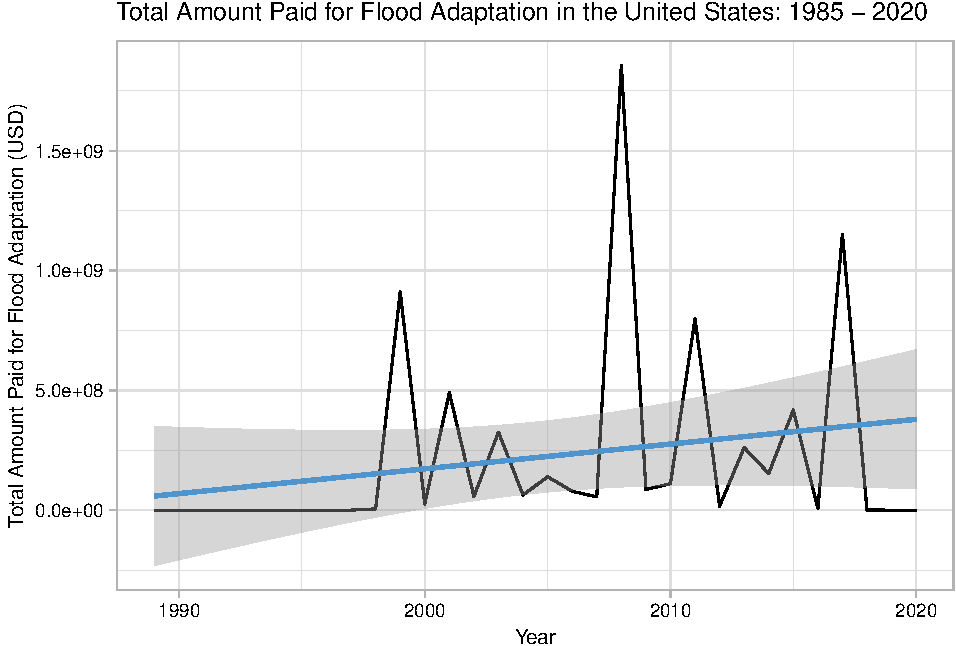
\includegraphics{finalreport_files/figure-latex/unnamed-chunk-11-1.pdf}
\caption{Total Amount Paid for Flood Adaptation between 1985 and 2020}
\end{figure}

However, after adjusting the total amount paid for each year for
inflation and thus making each value in 2020 dollars this trend was no
longer statistically significant (p = 0.568). This can be seen in figure
7 which shows the inflation adjusted values for total amount paid over
time.

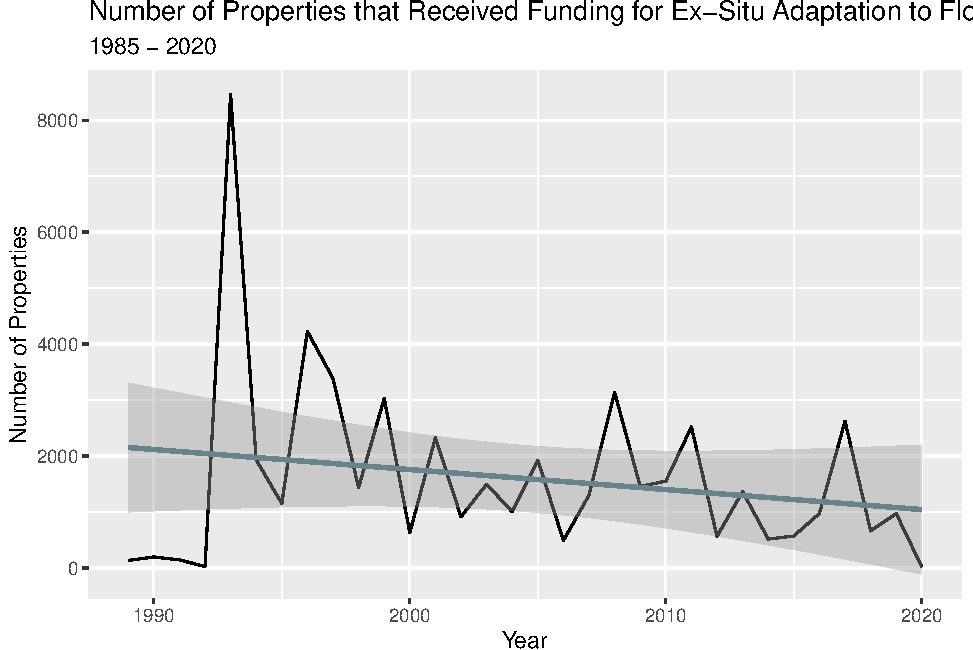
\includegraphics{finalreport_files/figure-latex/unnamed-chunk-12-1.pdf}
\newpage A summary of each of these time series results can be found in
table 3.

\emph{Table 3: Results from Time Series Analysis of All Adaptation
Types}\\
\captionsetup[table]{labelformat=empty,skip=1pt}

\begin{longtable}{lr}
\caption*{
{\large \emph{\textbf{Time Series Analysis Results: All Adaptation Types}}}
} \\ 
\toprule
Measure & Result \\ 
\midrule
\multicolumn{1}{l}{**Number of Properties**} \\ 
\midrule
Tau & $0.000$ \\ 
P-value & $1.000$ \\ 
\midrule
\multicolumn{1}{l}{**Total Amount Paid**} \\ 
\midrule
Tau & $0.087$ \\ 
P-value & $0.568$ \\ 
\midrule
\multicolumn{1}{l}{\textbf{Inflation Adjusted Total Amount Paid}} \\ 
\midrule
Tau & $0.087$ \\ 
P-value & $0.568$ \\ 
\bottomrule
\end{longtable}

These findings suggest that there is no statistically significant
monotonic trend in the number of properties that receive grants for
flooding adaptation nor the amount spent on flooding adaptation by the
Federal Emergency Management Agency. Though there was a trend in the
total amount paid, this trend was no longer present when adjusting for
inflation suggesting that the trend was likely a reflection of inflation
rather than of an increase in amount spent.

\hypertarget{ex-situ-adaptation}{%
\subsection{4.2 Ex-Situ Adaptation}\label{ex-situ-adaptation}}

The second analysis involved the three time series analyses identifying
possible monotonic trends in ex-situ adaptation between 1985 and 2020.
Again, the only statistically significant monotonic trend was the trend
in total amount paid for buyouts before adjusting for inflation. There
does appear to be a declining trend in the total number of properties
that received ex-situ funding from FEMA as seen in Figure 8, however,
the time series analysis reveals that this is not a statistically
significant trend (p = 0.57).

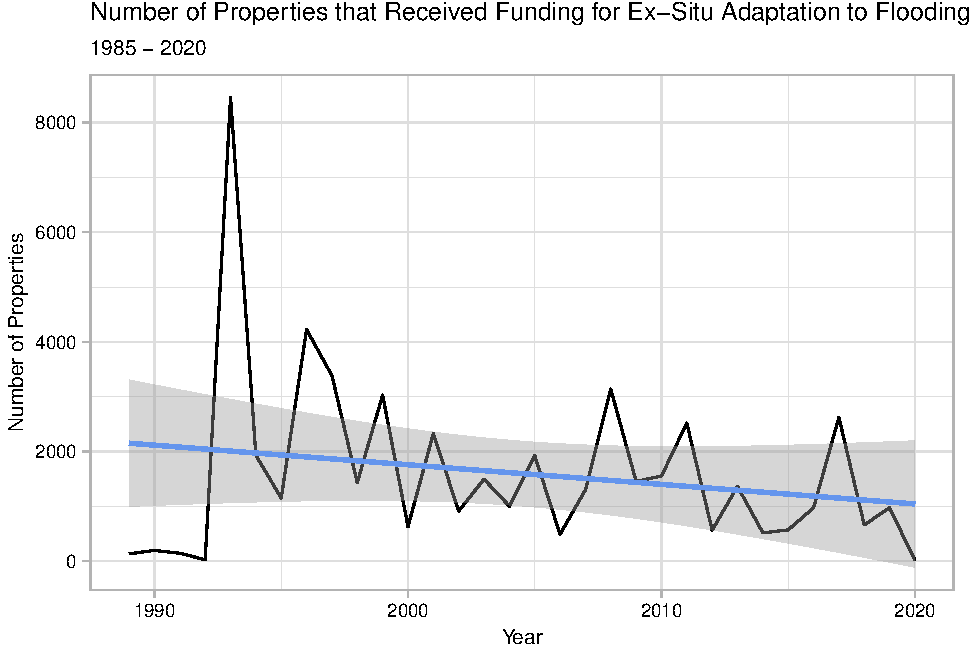
\includegraphics{finalreport_files/figure-latex/unnamed-chunk-15-1.pdf}
\newpage

The statistically significant monotonic trend in the total amount paid
for buyouts (p = 0.003) can be found in figure 9.

\begin{figure}
\centering
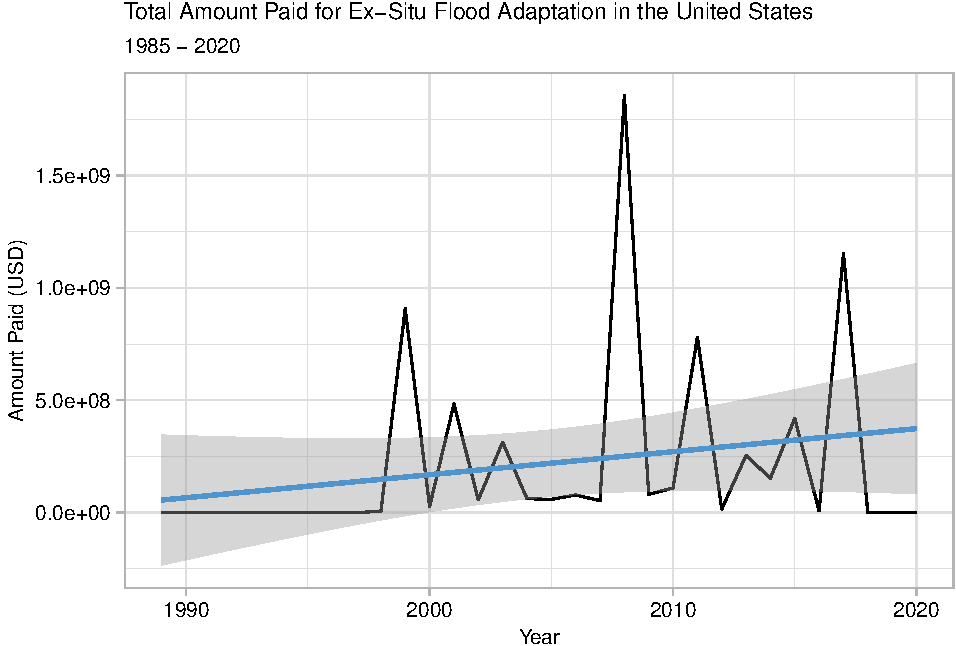
\includegraphics{finalreport_files/figure-latex/unnamed-chunk-16-1.pdf}
\caption{Total Amount Paid for Ex-Situ Adaptation to Flooding between
1985 and 2020}
\end{figure}

\newpage

However, after adjusting for inflation, again, the trend in total amount
paid was no longer found to be statistically significant with a p-value
of 0.503 after adjusting each total amount paid value to 2020 dollars.
Figure 10 shows the graph of this trendline and data over time.

\begin{figure}
\centering
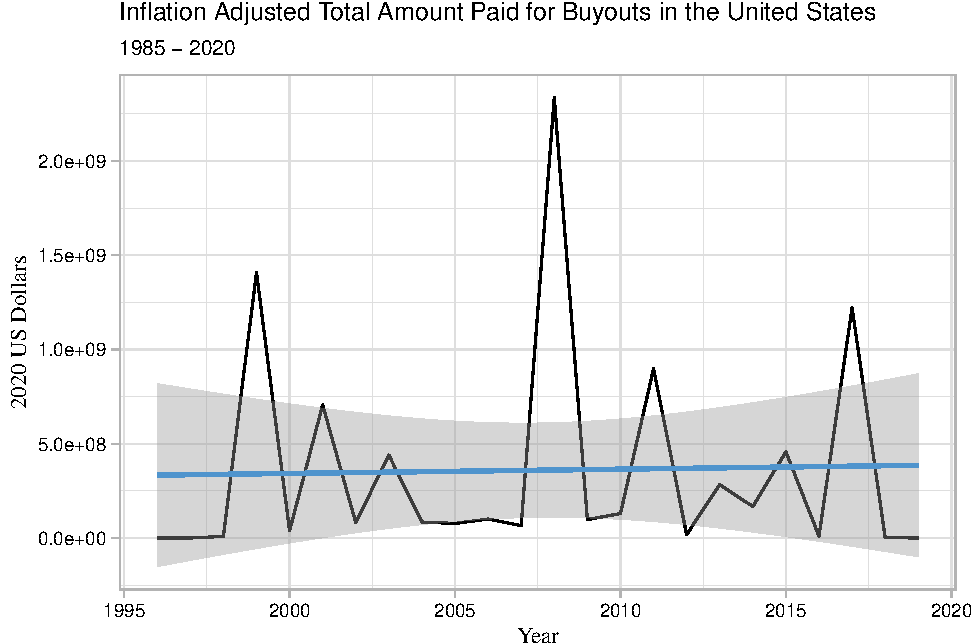
\includegraphics{finalreport_files/figure-latex/unnamed-chunk-17-1.pdf}
\caption{Total Amount Paid for Ex-Situ Adaptation to Flooding between
1985 and 2020 in 2020 Inflation Adjusted U.S. Dollars.}
\end{figure}

\newpage

A table of the results of all of these three analyses can be found in
table 4.

\emph{Table 4: Results from Time Series Analysis of Ex-Situ
Adaptation}\\
\captionsetup[table]{labelformat=empty,skip=1pt}

\begin{longtable}{lr}
\caption*{
{\large \emph{\textbf{Time Series Analysis Results: Ex-Situ Adaptation}}}
} \\ 
\toprule
Measure & Result \\ 
\midrule
\multicolumn{1}{l}{\textbf{Number of Properties}} \\ 
\midrule
Tau & $-0.073$ \\ 
P-value & $0.570$ \\ 
\midrule
\multicolumn{1}{l}{\textbf{Total Amount Paid}} \\ 
\midrule
Tau & $-0.073$ \\ 
P-value & $0.570$ \\ 
\midrule
\multicolumn{1}{l}{\textbf{Inflation Adjusted Total Amount Paid}} \\ 
\midrule
Tau & $0.101$ \\ 
P-value & $0.503$ \\ 
\bottomrule
\end{longtable}

These findings are consistent with the overall trends in all flooding
adaptation grants over time, suggesting that there is not a
statistically significant increase in ex-situ adaptation over time.
Again, the trend in the total amount spent was likely due to trends in
inflation rather than the actual amount spent as the trend was no longer
present when accounting for inflation in the final time series analysis.

\hypertarget{in-situ-analysis}{%
\subsection{4.3 In-Situ Analysis}\label{in-situ-analysis}}

The final time series analysis examined in-situ adaptation specifically,
which is adaptation in place that allows an individual to adapt their
property to the flooding through putting in a seawall, raising their
home, etc. Again these time series examined possible monotonic trends in
the number of properties and the total amount paid with and without
inflation adjustments between 1985 and 2020. There was again only one
statistically significant trend, however, for this analysis it was the
trend in the number of properties over time.

The number of properties that received in-situ adaptation funding was
found to have a statistically significant monotonic increasing trend (p
= 0.0004, tau = 0.44). This trend can be seen in figure 11.

\begin{figure}
\centering
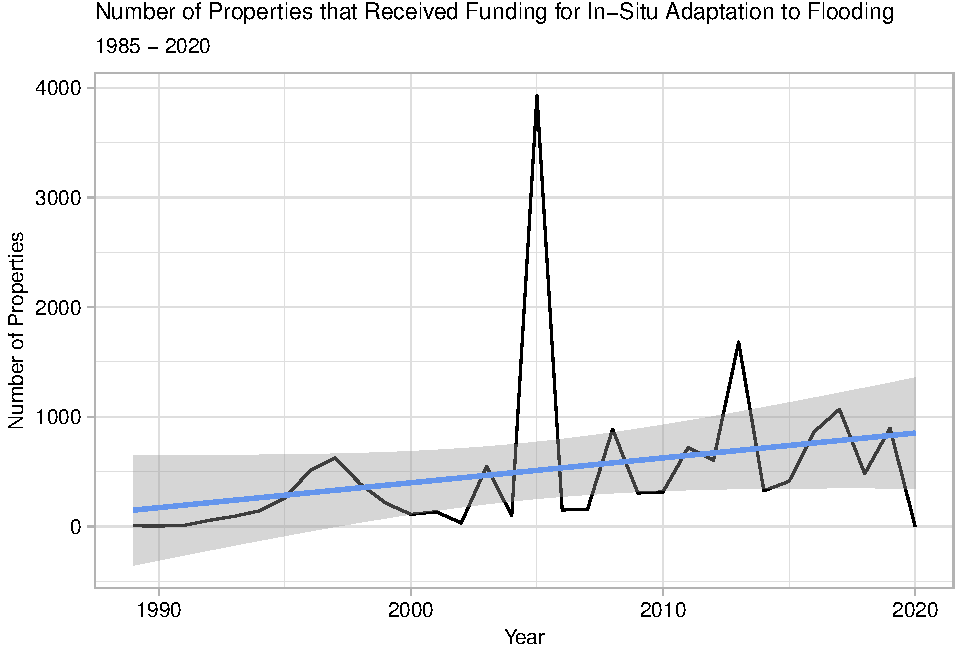
\includegraphics{finalreport_files/figure-latex/unnamed-chunk-20-1.pdf}
\caption{Number of Properties that Received Grant Funding for In-Situ
Adaptation to Flooding between 1985 and 2020.}
\end{figure}

The other two analyses, total amount paid and inflation adjusted total
amount paid, were not statistically significant with p-values of 0.207
and 0.484 respectively. The graphs showing this data over time with the
associated trend line can be seen in figures 12 and 13. Both graphs show
a drastic spike in payments in 2008 - this is likely due to Hurricane
Katrina where significant funding was needed to help communities in
Louisiana recover and adapt to these types of storms.

\newpage

\begin{figure}
\centering
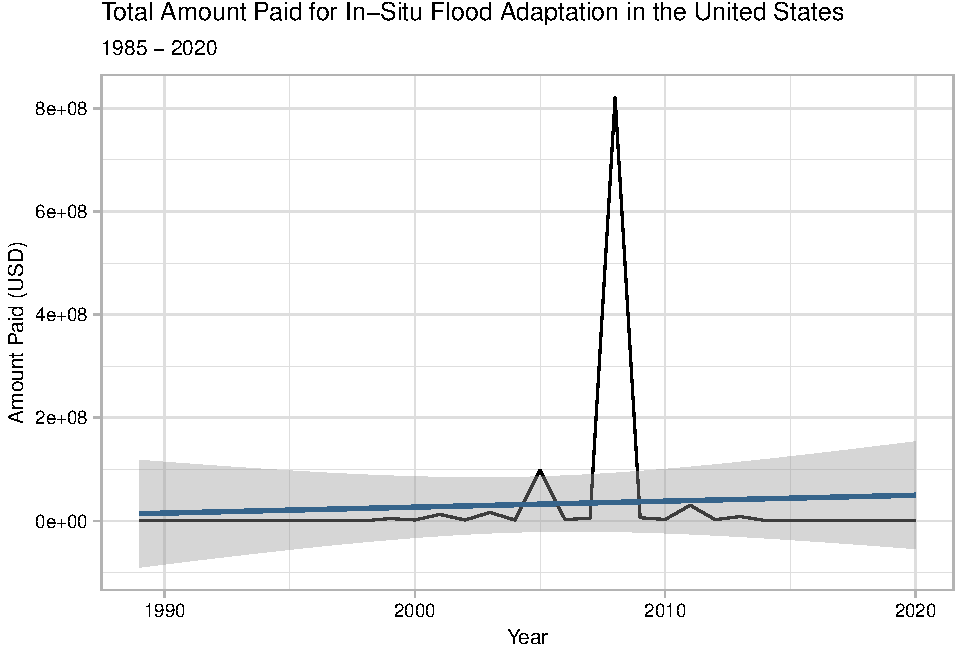
\includegraphics{finalreport_files/figure-latex/unnamed-chunk-21-1.pdf}
\caption{Total Amount Paid for In-Situ Adaptation to Flooding between
1985 and 2020.}
\end{figure}

\begin{figure}
\centering
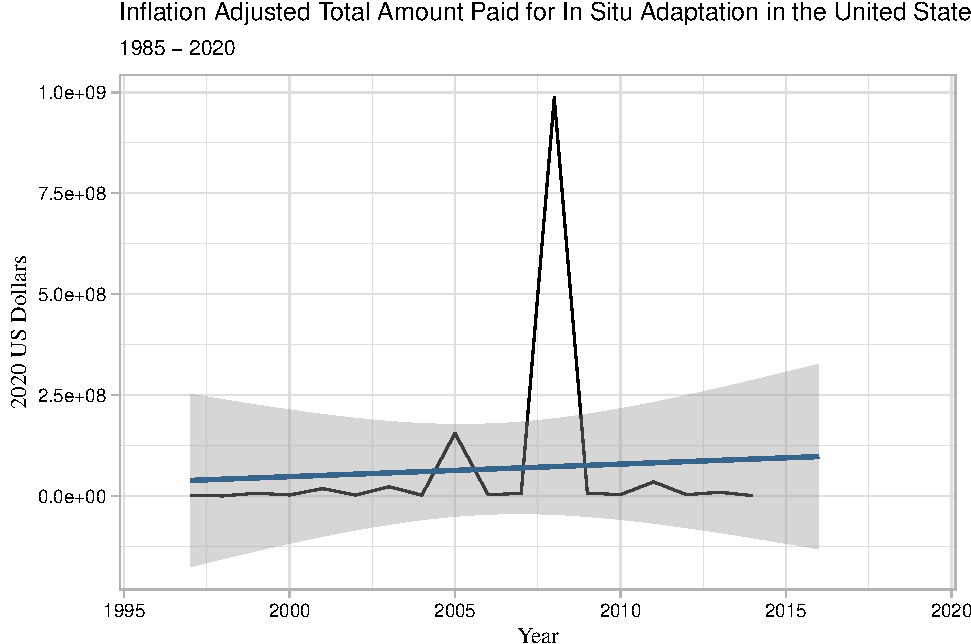
\includegraphics{finalreport_files/figure-latex/unnamed-chunk-22-1.pdf}
\caption{Total Amount Paid for In-Situ Adaptation to Flooding between
1985 and 2020 in 2020 Inflation Adjusted U.S. Dollars.}
\end{figure}

\newpage

A table of each of these time series results can be found in table 5.

\emph{Table 5: Results from Time Series Analysis of In-Situ
Adaptation}\\
\captionsetup[table]{labelformat=empty,skip=1pt}

\begin{longtable}{lr}
\caption*{
{\large \emph{\textbf{Time Series Analysis Results: In-Situ Adaptation}}}
} \\ 
\toprule
Measure & Result \\ 
\midrule
\multicolumn{1}{l}{\textbf{Number of Properties}} \\ 
\midrule
Tau & $0.440$ \\ 
P-value & $0.000$ \\ 
\midrule
\multicolumn{1}{l}{\textbf{Total Amount Paid}} \\ 
\midrule
Tau & $0.167$ \\ 
P-value & $0.207$ \\ 
\midrule
\multicolumn{1}{l}{\textbf{Inflation Adjusted Total Amount Paid}} \\ 
\midrule
Tau & $0.123$ \\ 
P-value & $0.484$ \\ 
\bottomrule
\end{longtable}

Overall, these findings suggest that more properties are receiving
in-situ adaptation funding, yet the total amount paid for in-situ
adaptation is not changing significantly. The increase in number of
properties is what one would expect given the increasing number of
people that are exposed to flooding over time. The lack of a paralleling
trend in total amount paid requires deeper analysis. It could be because
the measures are becoming more affordable as they are becoming more
common and necessary, or because more individuals are seeking more minor
in-situ adaptation projects. Deeper analysis on the exact type of
adaptation action would be necessary to understand why these trends
exist. Still, this analysis provides important insight that indicates
that there is a statistically significant increase in the number of
properties that are adapting in place to flooding impacts.

\hypertarget{spatial-analysis}{%
\subsection{4.4 Spatial Analysis}\label{spatial-analysis}}

The final part of this analysis sought to spatially visualize this data
as to explore possible spatial trends in the data to complement that
analysis of temporal trends. This spatial analysis specifically looked
at the data for North Carolina due to data availability and size. These
maps show the number of properties all adaptation, in-situ, and ex-situ
at the county level. The spatial analysis specifically showed the number
of properties rather than also or instead including the total amount
paid because the resulting maps were the same for both as the spatial
trends were consistent. Number of properties did not require inflation
adjustments and thus was selected over total amount paid for the
analysis.

First, Figure 14 helps to visualize where in North Carolina these
adaptation grants are concentrated by mapping the number of properties
that received flooding adaptation grants by county.

\begin{figure}
\centering
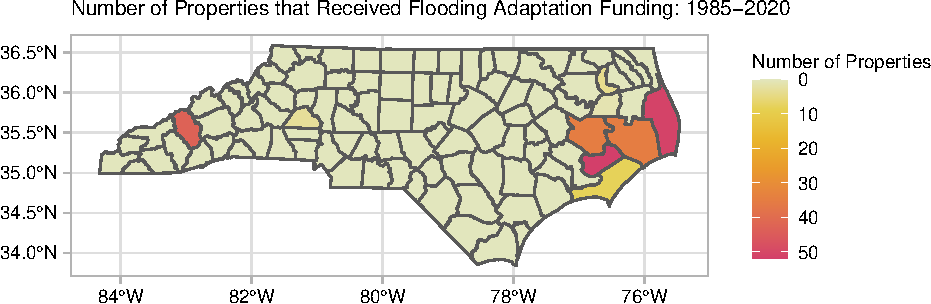
\includegraphics{finalreport_files/figure-latex/unnamed-chunk-26-1.pdf}
\caption{Spatial Distribution of the Number of Properties that Received
Flooding Adaptation Grant Funding between 1985 - 2020}
\end{figure}

\newpage

Figure 15 and 16 help to compare the areas that have a high number of
properties that received flooding adaptation grants for ex-situ
vs.~in-situ grants.

\begin{figure}
\centering
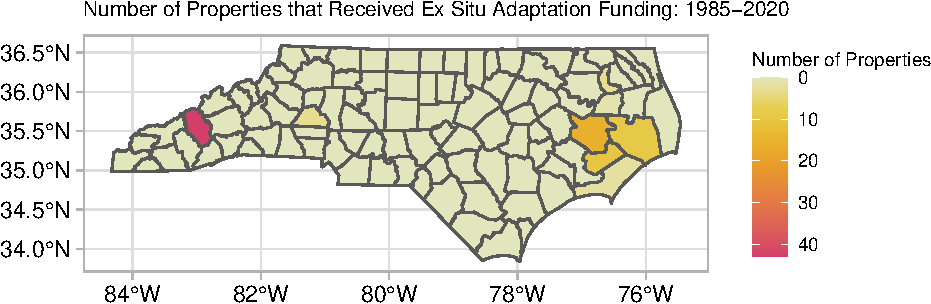
\includegraphics{finalreport_files/figure-latex/unnamed-chunk-27-1.pdf}
\caption{Spatial Distribution of the Number of Properties that Received
In-Situ Flooding Adaptation Grant Funding between 1985 - 2020}
\end{figure}

\begin{figure}
\centering
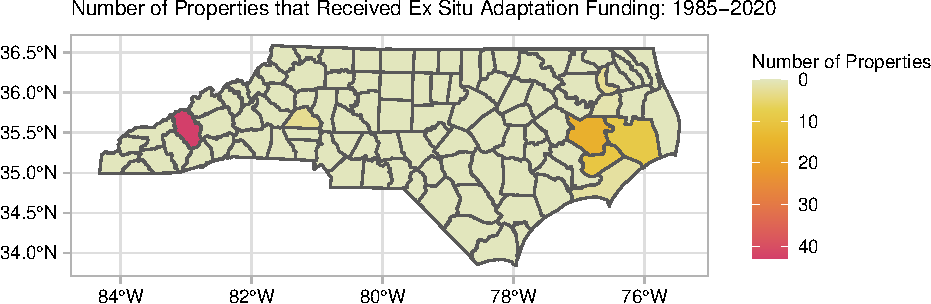
\includegraphics{finalreport_files/figure-latex/unnamed-chunk-28-1.pdf}
\caption{Spatial Distribution of the Number of Properties that Received
Ex-Situ Flooding Adaptation Grant Funding between 1985 - 2020}
\end{figure}

In comparing these two maps it is very clear that the ex-situ adaptation
funding is concentrated in the inland county whereas the in-situ
adaptation funding is concentrated on the coast. This is an important
finding, suggesting that buyouts occur more often inland likely from
riverine flooding whereas in-situ adaptation may be more common for
coastal flooding.

\newpage

\hypertarget{summary-and-conclusions}{%
\section{Summary and Conclusions}\label{summary-and-conclusions}}

\hypertarget{lack-of-overall-trends-in-flooding-adaptation}{%
\subsection{5.1 Lack of Overall Trends in Flooding
Adaptation}\label{lack-of-overall-trends-in-flooding-adaptation}}

For almost all of the time series analyses, we found no statistically
significant trend. This was true for trends in all adaptation types for
number of properties and total amount paid (after inflation
adjustments), as well as for buyouts for number of properties and total
amount paid (after inflation adjustments). There was also no
statistically significant trend in the total amount paid for in-situ
adaptation. This is inconsistent with the initial hypothesis that all of
these would be increasing due to the increase in flooding hazards across
the United States. However, a lack of a trend is still an important
finding in that it suggests that further analysis is needed to
understand why these resources are not being used. This could indicate
that despite potential increases in flooding, communities are not
experiencing this to the level that an adaptation measure would be
necessary. Alternatively, this could indicate that communities may just
not be aware of the resources that are available to them in the face of
flooding hazards. The lack of trends in buyouts may be a result of a
number of factors given the complicated nature of buyouts socially and
economically. Communities may be less apt to seek out a buyout because
of the challenges of moving, going through the bureaucratic process,
forming a new community, finding a new home, tc. and it may not be a
reflection of their exposure to hazard.

\hypertarget{trends-in-in-situ-flooding-adaptation-spatial-and-temporal}{%
\subsection{5.2 Trends in In-Situ Flooding Adaptation: Spatial and
Temporal}\label{trends-in-in-situ-flooding-adaptation-spatial-and-temporal}}

The only statistically significant trends, after adjusting the total
amount paid values for inflation, was the number of properties receiving
in-situ adaptation funding. In this case, again, the driver of this
trend is unknown. However, in considering this, the spatial analysis can
complement the interpretation of these findings. The spatial analysis
showed that the number of properties in North Carolina receiving in-situ
adaptation grants was heavily concentrated near the coast, while the
ex-situ adaptation properties were much more present inland from the
coast.

While there are many drivers of flooding and changes in flooding,
climate change has made the sea levels rise increasing coastal flooding
dramatically. If ex-situ adaptation primarily serves riverine flooding,
these grants would not be impacted by sea level rise trends. Similarly,
if in-situ funding primarily serves coastal communities one would expect
an increasing trend in in-situ grants associated with the increase in
sea level. This is reflected in our findings for both in-situ and
ex-situ trends in the number of properties over time, with the spatial
analyis providing insight on how to consider these findings. It is
possible that the increase in in-situ adaptation is associated with the
increase in sea level whereas the ex-situ adaptation funding is more
responsive to changes in inland flooding. However, this is just a
hypothesis based on the findings from this analysis. A nationwide
analysis of the spatial trends in in-situ vs.~ex-situ adaptation is
necessary to determine if this is consistent across the United States
and then a deeper analysis is necessary to identify drivers of these
trends such as sea level rise.

\hypertarget{opportunities-for-future-research}{%
\subsection{5.3 Opportunities for Future
Research}\label{opportunities-for-future-research}}

The findings from this analysis provided foundations for future research
on trends in adaptation funding in the United States. Extending the
spatial analysis to include the entirety of the United States would
allow an exploration of the trends in ex-situ and in-situ grants beyond
those in North Carolina to identify if these are representative of the
rest of the United States. Furthermore, deeper analysis that compare
these trends with those of sea level rise, as well as socio-economic
factors such as the cost of adaptation, would allow researchers to begin
to identify potential drivers of these trends.

\newpage

\hypertarget{references}{%
\section{References}\label{references}}

State of North Carolina. 2020. ``North Carolina State and County
Boundary Polygons.'' \emph{ArcGIS Hub.}
\url{https://hub.arcgis.com/datasets/NCEM-GIS}::north-carolina-state-and-county-boundary-polygons/about

Environmental Protection Agency. 2020. ``Climate Change Indicators:
Coastal Flooding.'' \emph{Climate Change Indicators.}
\url{https://www.epa.gov/climate-indicators/climate-change-indicators-coastal-flooding\#}:\textasciitilde:text=Data\%20\%7C\%20Technical\%20Documentation-,Key\%20Points,Coasts\%20(see\%20Figure\%202).

Internal Displacement Monitoring Centre (IDMC). 2019. ``United States of
America: Figure Analysis, Displacement Related to Disasters.''
\emph{IDMC.}
\url{https://www.internal-displacement.org/sites/default/files/inline-files/GRID-2019-Disasters-Figure-Analysis-UnitedStates.pdf}

Lindsey, R. 2022. ``Climate Change: Global Sea Level.''
\emph{Climate.gov.}
\url{https://www.climate.gov/news-features/understanding-climate/climate-change-global-sea-level}

Federal Emergency Management Agency (FEMA). 2022. ``OpeFEMA Dataset:
Hazard Mitigation Assistance Mitigated Properties - v2.'' \emph{Reports
\& Data.}
\url{https://www.fema.gov/openfema-data-page/hazard-mitigation-assistance-mitigated-properties-v2}

Wing O., Lehman, W., Bates, P., Sampson, C., Quinn, N., Smith, A., Neal,
J., Porter, J., \& Kousky, C. 2022. ``Inequitable patterns of US flood
risk in the Anthropocene.'' \emph{Nature} 12:
\url{https://www.nature.com/articles/s41558-021-01265-6}

\end{document}
